\documentclass[a4paper,12pt]{article}
\usepackage[english]{babel}
\usepackage{setspace}
\usepackage[backend=bibtex, style=chicago-authordate]{biblatex}
\usepackage{graphicx} %for graphics
\usepackage{hyperref} %for links
\graphicspath{ {/home/heidi/Gradu2_0/Images/} }
\addbibresource{mastersthesis.bib}


\begin{document}
\section{Method}
- computer aided network analysis <- distinction between 'verkostotutkimus' mentioned in Juuso Marttila's thesis. 
Quite a few textbooks have been written on network analysis.

Furthermore, in the field of technology network analysis does have some everyday application, such as the analysis of the internet. 

\subsection{Defining the network}
Network analysis is based on the mathematical graph theory. A graph is a representation of the network. Graph includes nodes and edges.

\begin{figure}[h]
	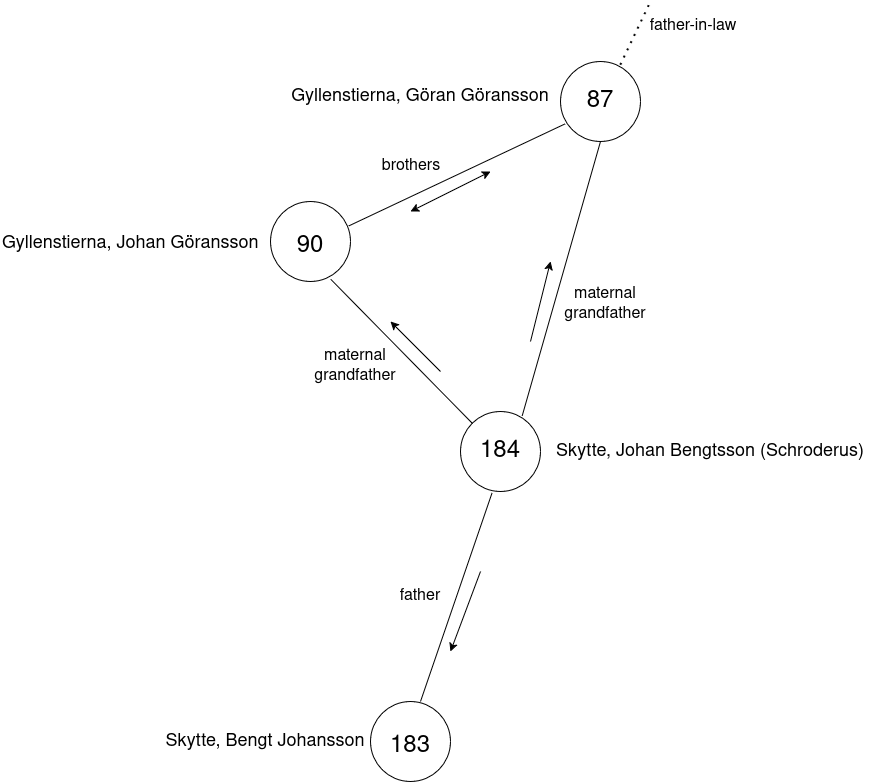
\includegraphics[scale=0.25]{example_network.drawio.png}
	\centering
	\caption{A sample from the graph} 
	\centering
\end{figure}
In this context the graph's nodes depict individual councillors with the input of name and id number. Correspondingly the edges represent the kinships between two nodes. For instance, in Figure 1 we can see that Johan Bengtsson (Schroderus) Skytte (id 184) is Bengt Johansson Skytte's (id 183) father and a maternal grandfather for Johan Göransson Gyllenstierna (id 90) and Göran Göransson Gyllenstierna (id 87). Johan Göransson and Göran Göransson are brothers, however, their father is not mentioned in the dataset. Göran Göransson also has further links in the network. \footfullcite{councillorsDS} 

\subsection{Implementation of the network analysis}
The data processing and analysis is conducted with a combination of Python programming language and Gephi software. Python is used for extracting the data from the councillors-dataset and formulating it in the right format: readable for Gephi. The actual network analysis, visualization and calculating statistics, is performed with Gephi. 

Python is a programming language commonly used in scientific work.
On my opinion simple syntax, easy to implement smaller tasks such as data processing. Readable, widely used therefore makes the work replicable. 

As graphs are structures commonly used in programming, it would have been possible to conduct the actual network analysis using tools provided by Python, yet, Gephi software provides a visual user interface and more intuitive tools for the manipulation of the graph.

Gephi is ...

Gephi is not always the most intiutive to use. Problems especially with node labels. \footnote{For Linux environments opening Gephi from command line with command "LIBGL\_ALWAYS\_SOFTWARE=1 ./gephi" can sometimes help.} 

Both of these tools are also open source and free to download.

All scripts written for this work available on GitHub(TODO link)

\subsubsection{Test run}
TODO add also to the source section about the end
TODO fix councillor / concilor typo

To draft the structure of the graph and understand the nuances of the given data a test run was carried out. The test run was done with a simple Python script, and no attention was paid to the temporal aspects of the network or the potential directions in the graph. The scripts and Gephi project of the test run is available in GitHub in the TestRun folder\footnote{Link: \url{https://github.com/Heidi-Suurkaulio/mastersthesis/tree/main/TestRun}}, the visualization of the test run graph can be found in the appendix (TODO put them there!)

The data processing was started by manually cleaning the data in LibreOffice Calc (equivalent to Microsoft Excel). The columns and rows containing information of the source material of the dataset and councillor's years active were removed. That made the structure of the data coherent and easier to manipulate with the Python script. The manually cleaned data is exported as .csv (comma separated values) file. The .csv file's header (the first line of the file) should be modified so that the column name "No." is changed to "Id" and "Family members in the council of the realm" is changed to "Family", the first one can cause an error if referenced in the Python code, the latter is inconveniently long. 

\begin{table}[h]
	\caption{Example of the raw .csv file}
	\resizebox{\textwidth}{!}{%
		\begin{tabular}{cccccccccp{1.5in}p{1.5in}}
			\hline
			1 &Name; &Id; &D.O.B.; &died; &Appointed; &Date; &Age; &Noble rank; &Family; &Spouse(s) / Father of Spouse / Date of Marriage \\
			\hline
			
			2 &Ingemar Petri; &162; &; &1530; &1495; &; &; &Estate unknown, Bishop; &; &; \\
			\hline
			3 &Tre Rosor, Ture Jönsson; &231; &; &1532; &1497; &; &; &Uradel (Ancient Nobility); &Father CR, Father-in-law CR, Sons 228, 230, Son (illegitimate) 175; &Anna Johansdotter/ Johan Christiernsson Vasa (CR) \\
			\hline
		\end{tabular}%
	}
\end{table}

The script itself reads the data from the .csv file. The connections between the councillors are separated from the "Family" column, based on the knowledge that each connection is marked with the id number of another councillor. The connections are then formatted and printed to .csv file. The connections .csv file containing values for "Source" id of the source concillor, "Target" id of target councillor, "Type" standard "Undirected", "Id" id number for the connection, "Weight" standard 1.0. Another .csv file is formatted and printed with the information of councillors' names and id numbers.

\begin{table}[h]
	\caption{Example of the connections .csv file}
	\centering
	\begin{tabular}{cccccc}
		\hline
		1 &Source, &Target, &Type, &Id, &Weight \\
		\hline
		2 &231, &228, &Undirected, &0, &1.0 \\
		\hline
		3 &231, &230, &Undirected, &1, &1.0 \\
		\hline
	\end{tabular}
\end{table}
\begin{table}[h]
	\caption{Example of the councillors .csv file}
	\centering
	\begin{tabular}{ccc}	
		\hline
		1 &Id; &Label \\
		\hline
		2 &162; &Ingemar Petri \\
		\hline
		3 &231; &Tre Rosor, Ture Jönsson \\
		\hline
	\end{tabular}
\end{table}

These .csv files are readable for Gephi. The outcome was an undirected graph of the councillors' affiliation network that had accumulated during the 160 years. The graph consisted of 261 nodes (257 real + 4 "ghosts") and 372 edges (including self loops and "ghost" nodes). The test run revealed three problems within the graph: the emergence of the empty "ghost" nodes, parallel edges and thirdly self loops. 

The "ghost" nodes were excess nodes with no name and only an id number and one or two connections in the graph. They were due to the references to the data points removed from the original dataset, and therefore can be ignored. The ghosts are discussed further in the subsection sources. However, the more essential problem are edge duplicates.

The edge duplicates occur because one relationship, such as father and son, is sometimes marked twice in the dataset. For example, in the case of Göran Göransson Gyllenstierna (id 87) the relatives are "Maternal Grandfather 184, Brother 90, Father-in-law 3, ...", and the parallel relationship is found in his grandfather's Johan Bengtsson (Schroderus) Skytte's (id 184) links: "Son 183, Grandson through daughter 87". Yet, the connection to Göran Göransson's brother Johan Göransson Gyllenstierna (id 90) is not marked in the grandfathers links. This means that the node of Göran Göransson Gyllenstierna (id 87) has one excess link compared to his brother's node. 

\begin{figure}[h]
	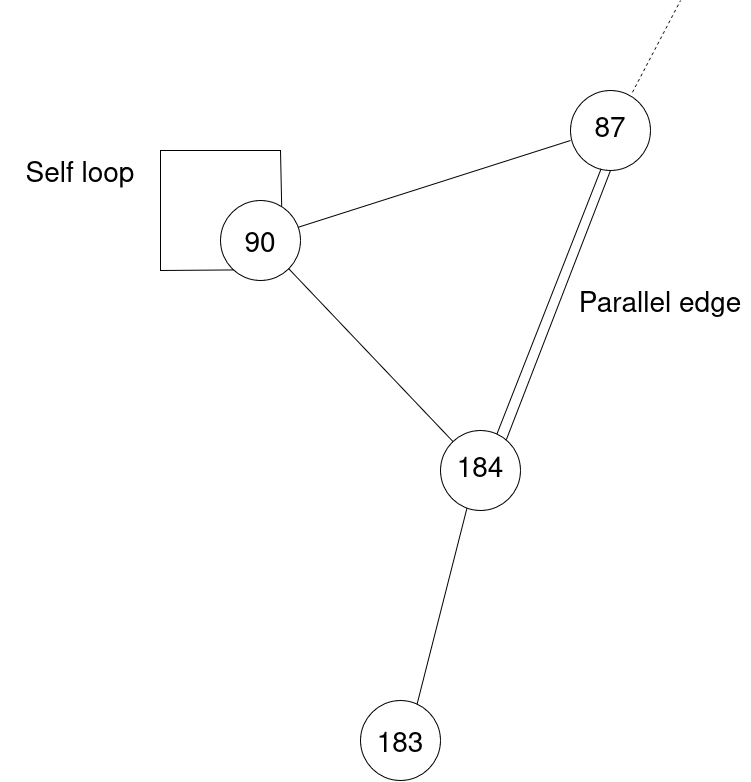
\includegraphics[scale=0.20]{double_link.drawio.png}
	\centering
	\caption{Visualisation of the parallel edge and self loop} 
	\centering
\end{figure}

The duplicate edges will cause bias to the calculation of the node degrees (TODO and other statistics)

Yifan Hu (default parameters except theta 2.0), noOverlap, manual checking and modification 

self loops t.ex. 90 to 90 or 5 to 5

the test run and "first look " PDF
test run problem: ghosts, duplicate connections(?)

Problems: we don't have data about the women

\end{document}
